\documentclass{article}
\usepackage{minted}
\usepackage{cleveref}
\usepackage{graphicx}
\usepackage{listings}
\usepackage{courier}
\usepackage[backend=biber,citestyle=authoryear,url=true,backref=bibtex,bibstyle=apa,useprefix=true]{biblatex}
\setminted[python]{fontfamily=courier}

\addbibresource{bibliography.bib}
\begin{document}
	\section{Source code}\label{sec:code} % (fold)
	The source code of this application, in its entirety can be found below, split up as follows: 
	\begin{itemize}
		\item Main source code 
		\item Facilities
		\item Exceptions
		\item Comparators
	\end{itemize}

	\subsection{Main source code}\label{sub:main_source_code} % (fold)
	\textit{MedicalConsole.java}
	\inputminted{java}{src/main/java/com/yvesstraten/medicalconsole/MedicalConsole.java}

	\pagebreak

	\textit{Format.java}
	\inputminted{java}{src/main/java/com/yvesstraten/medicalconsole/Format.java}

	\textit{Input.java}
	\inputminted{java}{src/main/java/com/yvesstraten/medicalconsole/Input.java}

	\textit{ArrayListSet.java}
	\inputminted{java}{./src/main/java/com/yvesstraten/medicalconsole/ArrayListSet.java}

	\textit{Editable.java}
	\inputminted{java}{src/main/java/com/yvesstraten/medicalconsole/Editable.java}

	\pagebreak

	\textit{HealthService.java}
	\inputminted{java}{src/main/java/com/yvesstraten/medicalconsole/HealthService.java}

	\textit{IdGenerator.java}
	\inputminted{java}{src/main/java/com/yvesstraten/medicalconsole/IdGenerator.java}
	% subsection Main source code (end)

	\subsection{Facilities}\label{sub:facilities} % (fold)
	\textit{Clinic.java}
	\inputminted{java}{src/main/java/com/yvesstraten/medicalconsole/facilities/Clinic.java}

	\pagebreak

	\textit{Hospital.java}
	\inputminted{java}{src/main/java/com/yvesstraten/medicalconsole/facilities/Hospital.java}

	\textit{MedicalFacility.java}
	\inputminted{java}{src/main/java/com/yvesstraten/medicalconsole/facilities/MedicalFacility.java}

	\textit{Procedure.java}
	\inputminted{java}{src/main/java/com/yvesstraten/medicalconsole/facilities/Procedure.java}

	\textit{Patient.java}
	\inputminted{java}{src/main/java/com/yvesstraten/medicalconsole/Patient.java}
	% subsection Facilities (end)

	\pagebreak
	
	\subsection{Comparators}\label{sub:comparators} % (fold)
	\textit{MedicalFacilitiesComparators.java}
	\inputminted{java}{src/main/java/com/yvesstraten/medicalconsole/comparators/MedicalFacilitiesComparators.java}

	\textit{PatientComparators.java}
	\inputminted{java}{src/main/java/com/yvesstraten/medicalconsole/comparators/PatientComparators.java}

	\textit{ProcedureComparators.java}
	\inputminted{java}{src/main/java/com/yvesstraten/medicalconsole/comparators/ProcedureComparators.java}
	% subsection Comparators (end)

  \newpage

	\subsection{Exceptions}\label{sub:exceptions} % (fold)
	\textit{ClassIsNotEditableException.java}
	\inputminted{java}{src/main/java/com/yvesstraten/medicalconsole/exceptions/ClassIsNotEditableException.java}

	\textit{InvalidOptionException.java}
	\inputminted{java}{src/main/java/com/yvesstraten/medicalconsole/exceptions/InvalidOptionException.java}

	\textit{InvalidYesNoException.java}
	\inputminted{java}{src/main/java/com/yvesstraten/medicalconsole/exceptions/InvalidYesNoException.java}

	\textit{NegativeNumberException.java}
	\inputminted{java}{src/main/java/com/yvesstraten/medicalconsole/exceptions/NegativeNumberException.java}

	\textit{NoHospitalsAvailableException.java}
	\inputminted{java}{src/main/java/com/yvesstraten/medicalconsole/exceptions/NoHospitalsAvailableException.java}

	\textit{WrongHospitalException.java}
	\inputminted{java}{src/main/java/com/yvesstraten/medicalconsole/exceptions/WrongHospitalException.java}
	% subsection Exceptions (end)

	\section{Unit tests}\label{sec:unit_tests} % (fold)
	For this assignment, unit tests written in JUNIT 5 \textcite{Junit5} were used extensively. Each unit test is show as follows:
	
	\textit{AddTests.java} 
	\inputminted{java}{src/test/java/com/yvesstraten/medicalconsole/tests/AddTests.java}

	\textit{ClinicTests.java} 
	\inputminted{java}{src/test/java/com/yvesstraten/medicalconsole/tests/ClinicTests.java}

	\textit{DeleteTests.java} 
	\inputminted{java}{src/test/java/com/yvesstraten/medicalconsole/tests/DeleteTests.java}

	\textit{EditTests.java} 
	\inputminted{java}{src/test/java/com/yvesstraten/medicalconsole/tests/EditTests.java}

	\textit{FacilitiesTests.java} 
	\inputminted{java}{src/test/java/com/yvesstraten/medicalconsole/tests/FacilitiesTests.java}

	\textit{FormatTests.java} 
	\inputminted{java}{src/test/java/com/yvesstraten/medicalconsole/tests/FormatTests.java}

	\textit{HealthServiceTests.java} 
	\inputminted{java}{src/test/java/com/yvesstraten/medicalconsole/tests/HealthServiceTests.java}

	\textit{HospitalTests.java} 
	\inputminted{java}{src/test/java/com/yvesstraten/medicalconsole/tests/HospitalTests.java}

	\textit{MedicalConsoleTest.java} 
	\inputminted{java}{src/test/java/com/yvesstraten/medicalconsole/tests/MedicalConsoleTest.java}

	\textit{MedicalConsoleTests.java} 
	\inputminted{java}{src/test/java/com/yvesstraten/medicalconsole/tests/MedicalConsoleTests.java}

	\textit{PatientTests.java} 
	\inputminted{java}{src/test/java/com/yvesstraten/medicalconsole/tests/PatientTests.java}

	\textit{ProcedureTests.java} 
	\inputminted{java}{src/test/java/com/yvesstraten/medicalconsole/tests/ProcedureTests.java}

	\textit{SortingTest.java} 
	\inputminted{java}{src/test/java/com/yvesstraten/medicalconsole/tests/SortingTest.java}

	When running these tests with \textit{mvn test} the following output is shown:
	\begin{figure}
		\begin{center}
			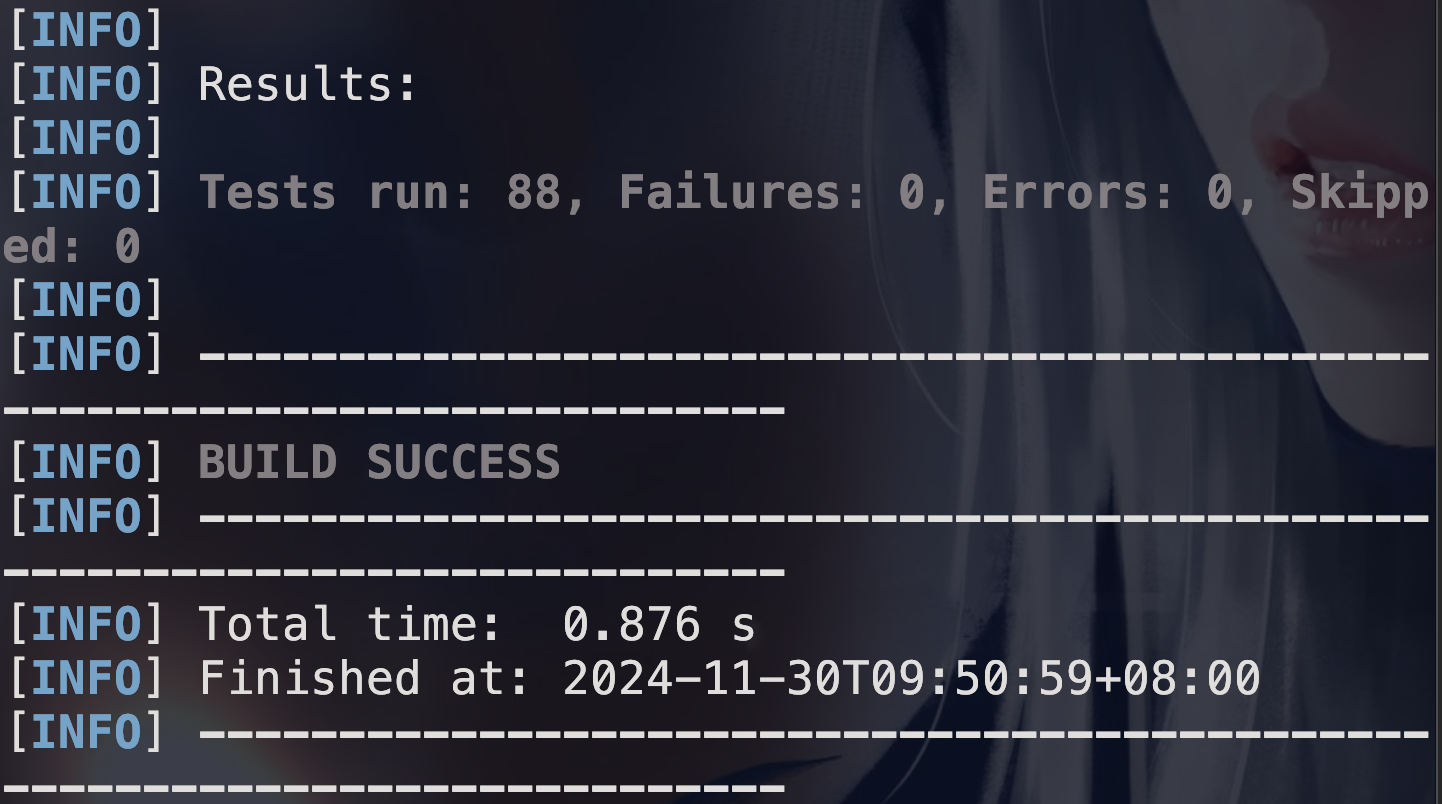
\includegraphics[width=0.8\textwidth]{figures/Mvn_test.png}
		\end{center}
		\caption{Test output}\label{fig:}
	\end{figure}
	
	% section Unit tests (end)

	\section{Runtime output}\label{sec:runtime_output} % (fold)
	Several runtime tests have been undertaken as well to test all functions of the program. These are:
	\begin{itemize}
		\item Adding objects
		\item Deleting objects 
		\item Sorting objects 
		\item Deleting objects
	\end{itemize}

	\subsection{Adding objects}\label{sub:adding_objects} % (fold)
	In this test, addition of objects will be tested with random misinputs to also check for the robustness of the system.


	% subsection Adding objects (end)
	
	% section Runtime output (end)

	\section{Bibliography}\label{sec:bibliography} % (fold)
	\printbibliography
	% section Bibliography (end)

\end{document}
